\documentclass[../document.tex]{subfiles}
\begin{document}\label{ssec:time}

%Use Roman numerals for sub-figures in this section
\renewcommand{\thesubfigure}{\roman{subfigure}}
\captionsetup[subfigure]{skip=-5pt}
\begin{figure}
    \begin{tabular}{lr}
        \subcaptionbox{{\bf kmeans} \label{fig:time-kmeans}}{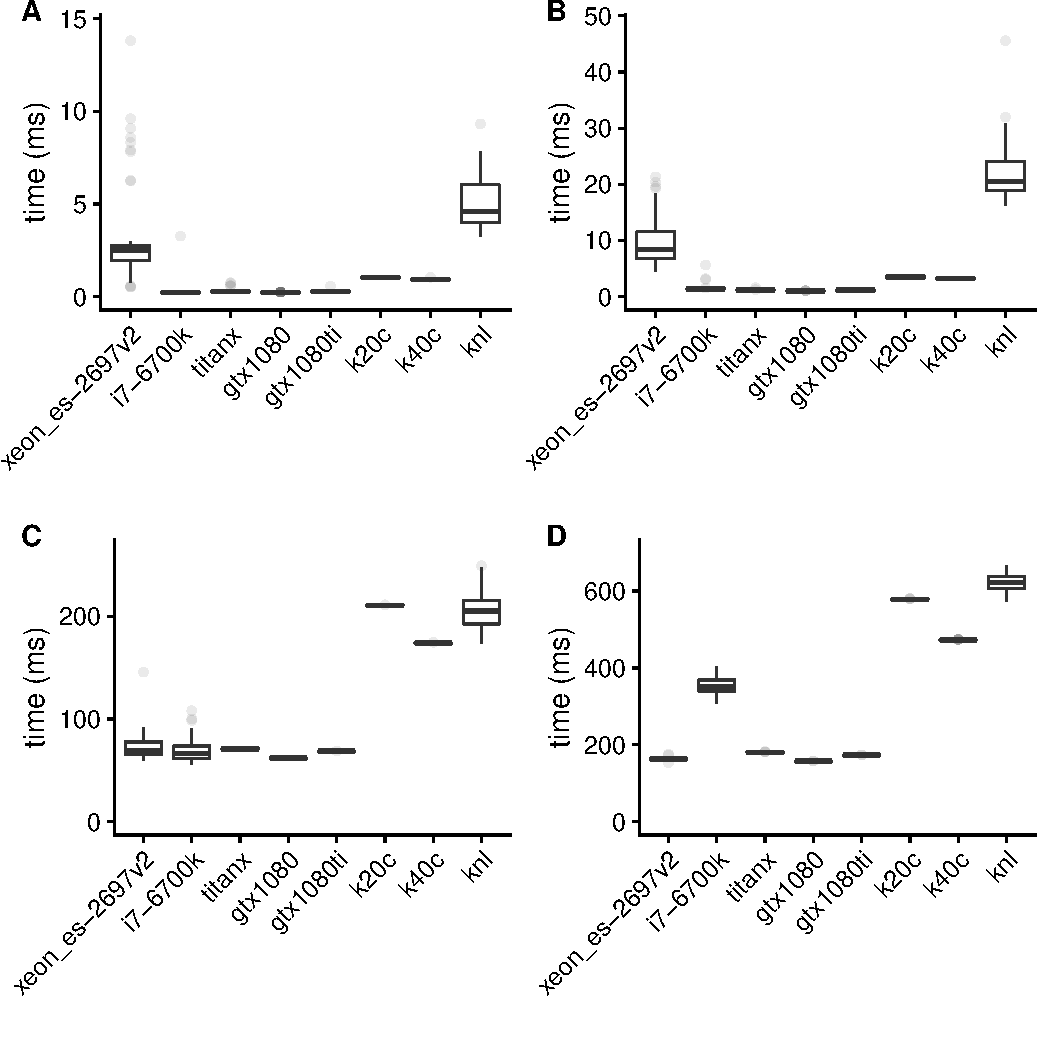
\includegraphics[width=.5\textwidth]{figures/time-results/kmeans.pdf}} &
        \subcaptionbox{{\bf lud} \label{fig:time-lud}}{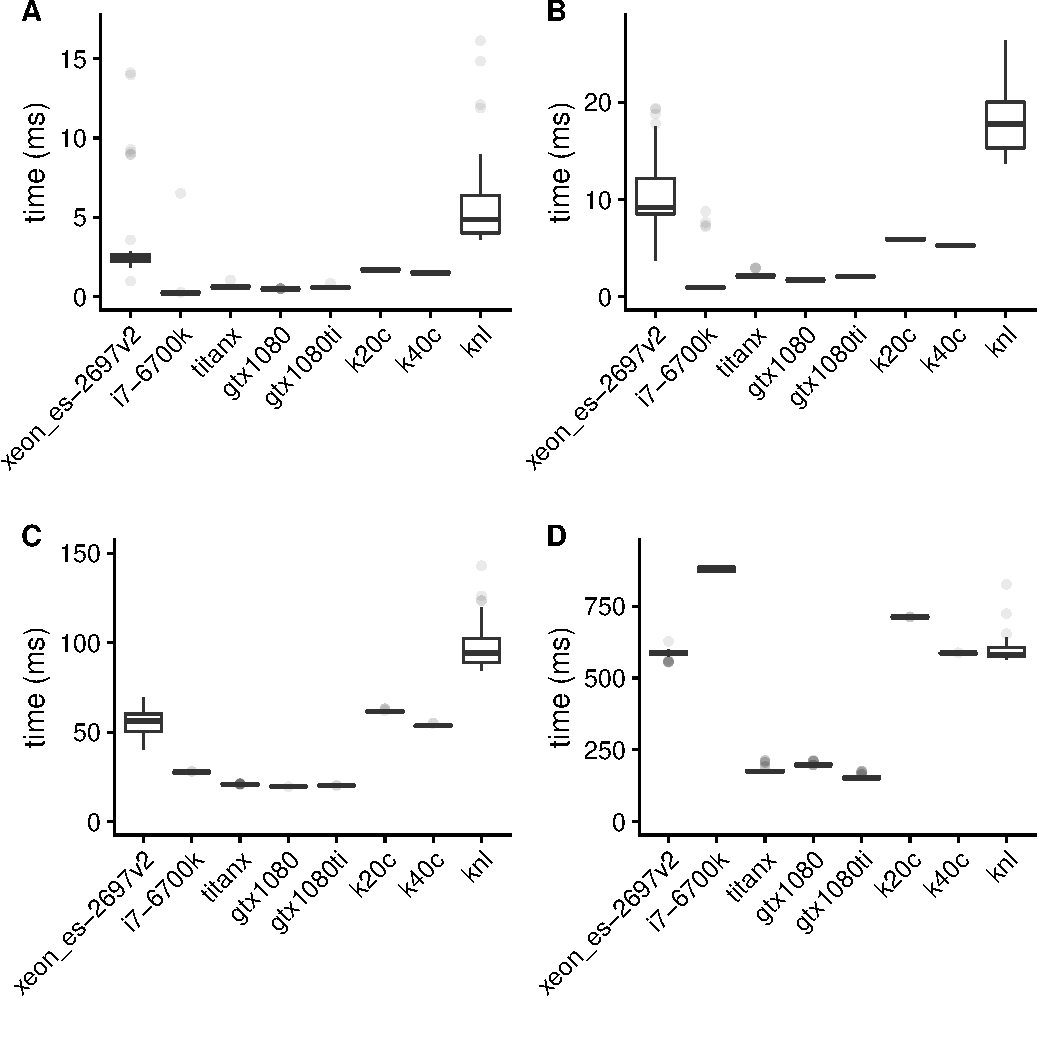
\includegraphics[width=.5\textwidth]{figures/time-results/lud.pdf}} \\
        \subcaptionbox{{\bf dwt} \label{fig:time-dwt}}{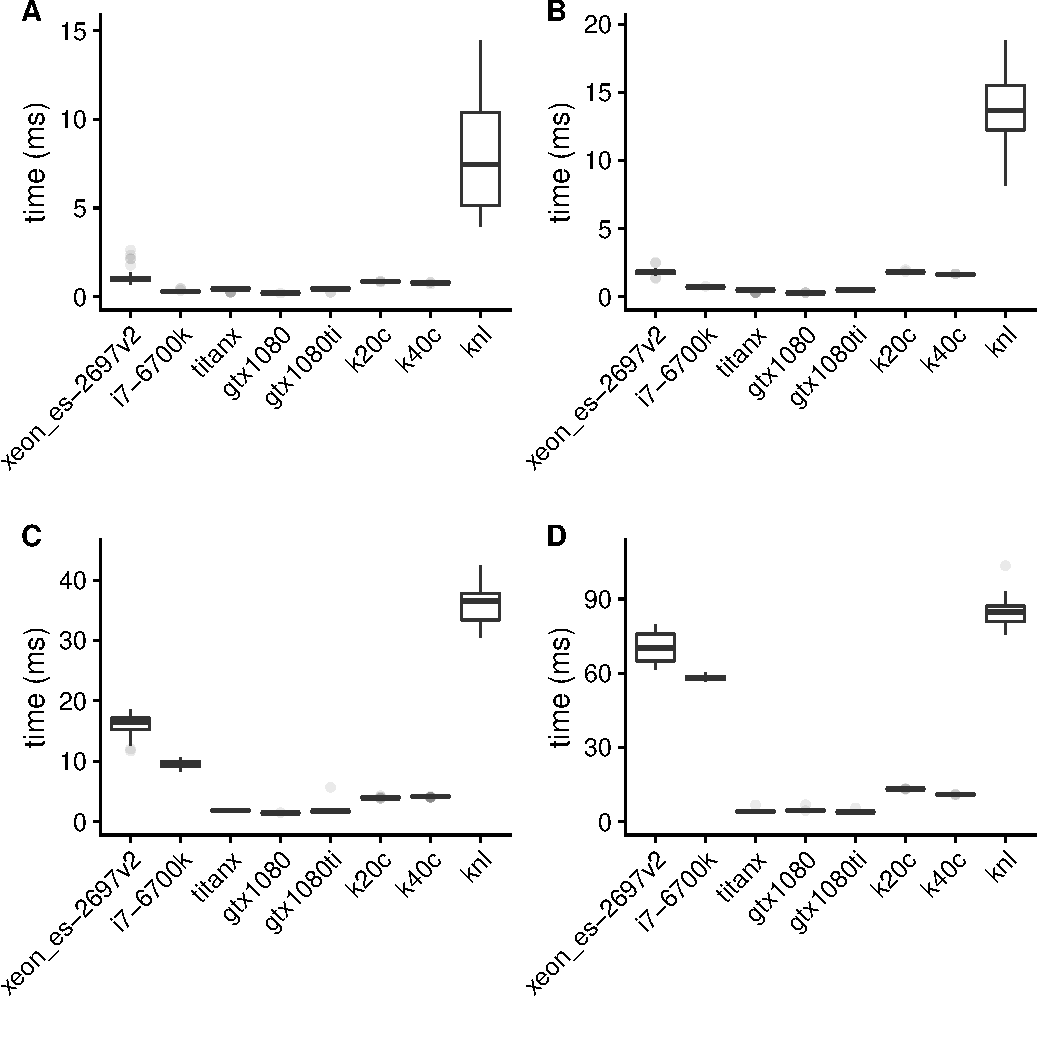
\includegraphics[width=.5\textwidth]{figures/time-results/dwt.pdf}} &
        \subcaptionbox{{\bf fft} \label{fig:time-fft}}{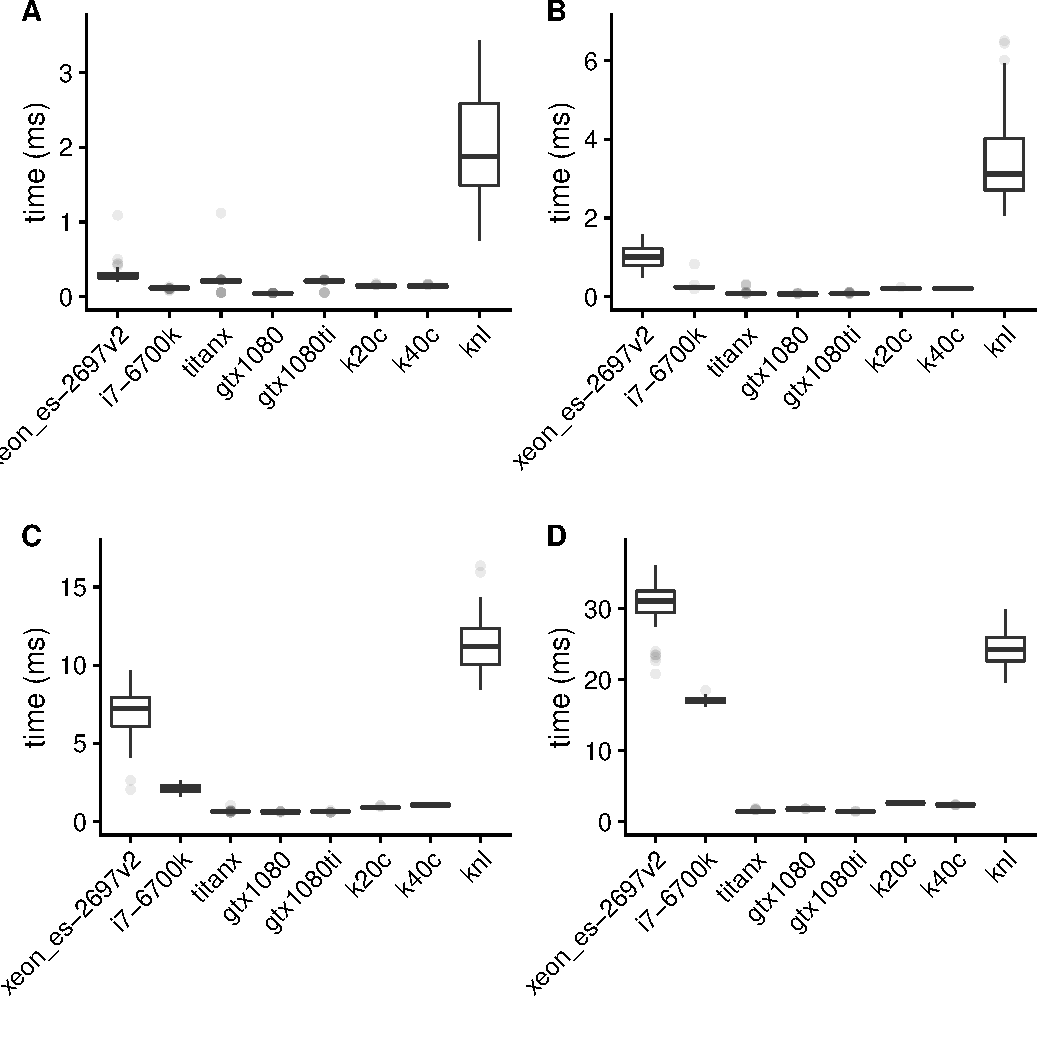
\includegraphics[width=.5\textwidth]{figures/time-results/fft.pdf}} \\
        \subcaptionbox{{\bf gem} \label{fig:time-gem}}{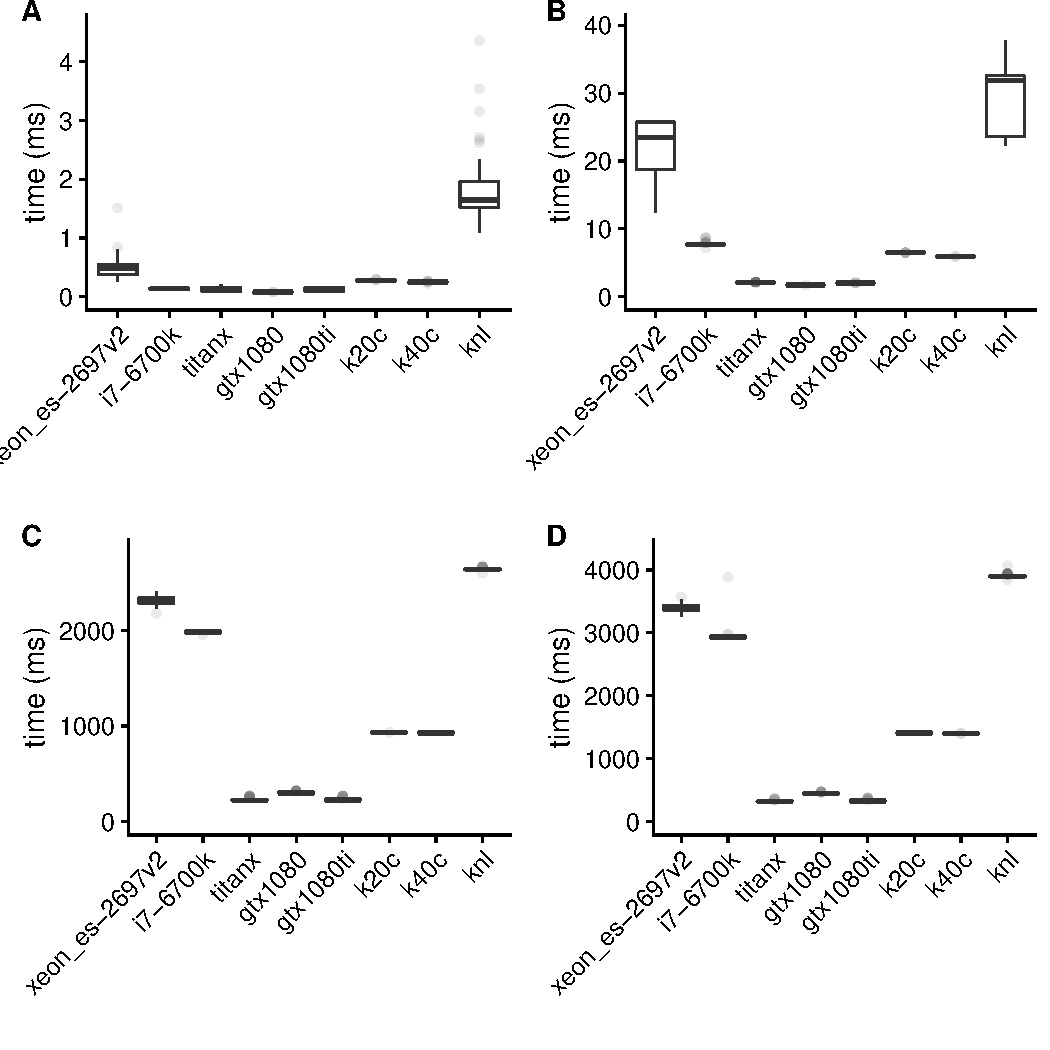
\includegraphics[width=.5\textwidth]{figures/time-results/gem.pdf}} &
        \subcaptionbox{{\bf srad} \label{fig:time-srad}}{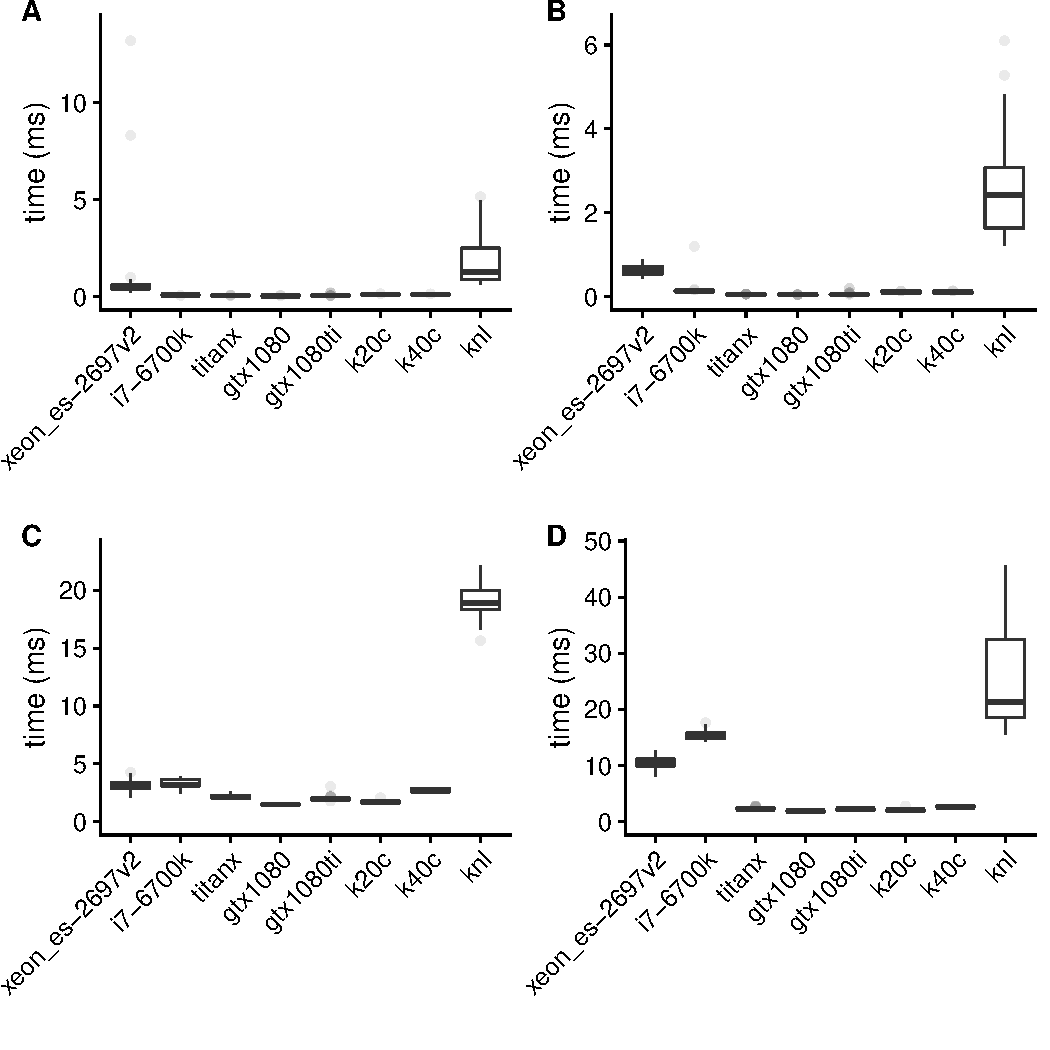
\includegraphics[width=.5\textwidth]{figures/time-results/srad.pdf}} \\
    \end{tabular}
    \caption{Kernel execution times for applications where the GPU architectures are optimal}
\end{figure}

Sample execution times from running 50 iterations per benchmark application.
LibSciBench has a high resolution timer with one cycle resolution and roughly \SI{6}{\nano\second} of overhead.
The top-left corner captions in all figures correspond to the 4 different workload sizes, such that {\bf A} corresponds to {\bf tiny}, {\bf B} corresponds to {\bf small}, {\bf C} to {\bf medium} and {\bf D} to {\bf large}.

The first two sets of figures in a row have applications which both correspond to a particular dwarf, for instance Figure~\ref{fig:time-kmeans} and Figure~\ref{fig:time-lud} are both representative of the Dense Linear Algebra dwarf, whereas Figure~\ref{fig:time-dwt} and Figure~\ref{fig:time-fft} are both applications within Spectral Methods.

Figure~\ref{fig:time-gem} represents N-Body Methods, Figure~\ref{fig:time-srad} encompasses a Structured Grid Method of Dwarf, and finally Figure~\ref{fig:time-crc} is a problem from Combinational Logic.
All but the {\bf crc} benchmark perform best on GPU type accelerators.

\todo{Are there any benchmarks where increasing the problem sizes makes results worse for the GPU?}
\todo{How does changing problem sizes affect benchmark performance across a range of platforms (selected accordingly to cache size)?}
\todo{Comment on the similarities within a dwarf and the differences between them.}

\end{document}
